\documentclass[twoside,numberorder]{csbachelor}
%==============================================================
%==============================================================

\usepackage{url}
\usepackage{subfigure}

%一些全局工具的定义
\DeclareMathOperator*{\argmin}{arg\,min}
\DeclareMathOperator*{\argmax}{arg\,max}

%==============================================================
%==============================================================
\begin{document}
%==============================================================
%==============================================================

  %论文题目:{中文}{英文}
  \zjutitle{}%
           {}
  %作者:{中文姓名}{英文}{学号}
  \zjuauthor{}{}{}
  %指导教师:{导师中文名}{导师英文名}
  \zjumentor{}{}
  %个人信息:{年级}{专业名称}
  \zjuinfo{}{}
  %学院信息:{学院中文}{学院英文}
  \zjucollege{}{}
  %日期:{Submitted Date}
  \zjudate{}

%==============================================================

  %封面
  %%============================================================
%% 中文封面

\thispagestyle{empty}

\vspace{5mm}

\begin{center}
   
\includegraphics[width=108mm]{images/zjdx}
\end{center}

\centerline{\songti\erhao\textbf{本科生毕业论文}}

\vspace{4mm}

\begin{center}
  
\includegraphics[width=35mm]{images/standxb}
\end{center}

\vspace{25mm}

{\hspace{16mm}\songti\sanhao\bfseries 题目:
  \hspace{2mm} \begin{minipage}[t]{98mm}\linespread{1.1}\uline{\zjutitlec}\end{minipage}}

\vspace{7mm}

\begin{tabbing}
    \hspace{30mm} \= \songti\sihao 姓\hspace{10mm}名: \= \underline{\makebox[6cm]{\sihao\zjuauthornamec\hspace{3mm}\zjuauthorid}} \\[2mm]
    \> \songti\sihao 学\hspace{10mm}号: \> 
    \underline{\makebox[6cm]{\sihao\zjuauthornamec}} \\[2mm]
              \> \songti\sihao 指导教师: \> \underline{\makebox[6cm]{\sihao\zjumentorc}} \\[2mm]
              \> \songti\sihao 专\hspace{10mm}业: \= \underline{\makebox[6cm]{\sihao\zjugrade\hspace{3mm}\zjumajor}} \\[2mm]
              \> \songti\sihao 学\hspace{10mm}院: \> \underline{\makebox[6cm]{\sihao\zjucollegec}}
\end{tabbing}


%%============================================================
% empty page for two-page print
\ifthenelse{\equal{\zjuside}{T}}{%
  \newpage\mbox{}%
  \thispagestyle{empty}}{}

%%============================================================
%% English Cover
\newpage
\thispagestyle{empty}

\vspace{5mm}

\begin{center}
    \songti\xiaoyi A Dissertation Submitted to Zhejiang University for the Degree of Bachelor of Engineering
\end{center}

\vspace{4mm}

\begin{center}
  
\includegraphics[width=35mm]{images/standxb}
\end{center}

\vspace{25mm}

{\hspace{3mm}\songti\sanhao\bfseries TITLE:\hspace{4mm}\begin{minipage}[t]{124mm}\linespread{1.1}{\renewcommand\baselinestretch{0.9}\selectfont\uline{\zjutitlee}\par}\end{minipage}}

\vspace{7mm}

\begin{tabbing}
    \hspace{18mm} \= \sanhao Author:\hspace{19mm} \= \underline{\makebox[8cm]{\sanhao\zjuauthornamee\hspace{3mm}\zjuauthorid}} \\[2mm]
                  \> \sanhao Supervisor: \> \underline{\makebox[8cm]{\sanhao\zjumentore}} \\[2mm]
                   \> \sanhao Major: \> \underline{\makebox[8cm]{\sanhao{Computer Science and Technology}}} \\[2mm]
                  \> \sanhao College: \> \underline{\makebox[8cm]{\sanhao\zjucollegee}} \\[2mm]
                  \> \sanhao Submitted Date: \> \underline{\makebox[8cm]{\sanhao\zjusubmitteddatee}}
\end{tabbing}

%%============================================================
% empty page for two-page print
\ifthenelse{\equal{\zjuside}{T}}{%
  \newpage\mbox{}%
  \thispagestyle{empty}}{}

  %诚信承诺书
  %% 诚信承诺书

\newpage
\thispagestyle{empty}

\begin{center}
\heiti\xiaosan 浙江大学本科生毕业论文(设计)诚信承诺书
\end{center}

\vspace{5mm}

{\songti\sihao
\begin{enumerate}
  \item 本人郑重地承诺所呈交的毕业论文(设计),是在指导教师的指导下严格按照学校和学院有关规定完成的。
  \item 本人在毕业论文(设计)中引用他人的观点和参考资料均加以注释和说明。
  \item 本人承诺在毕业论文(设计)选题和研究内容过程中没有抄袭他人研究成果和伪造相关数据等行为。
  \item 在毕业论文(设计)中对侵犯任何方面知识产权的行为,由本人承担相应的法律责任。
\end{enumerate}

\vspace{12mm}
\hspace{20mm}毕业论文(设计)作者签名:
\begin{flushright}
    \underline{\hspace{4em}} 年 \underline{\hspace{2em}} 月 \underline{\hspace{2em}} 日
\end{flushright}}

\ifthenelse{\equal{\zjuside}{T}}{%
  \newpage\mbox{}%
  \thispagestyle{empty}}{}


  \frontmatter
  \pagenumbering{Roman}

  %中文摘要
  %% 中文摘要
\chapter*{\centerline{摘\quad 要}}
\chaptermark{摘要}
\addcontentsline{toc}{chapter}{摘要}

\vspace{1em}
随着深度学习的发展,智能驾驶成为了火热的话题,而其中的一个字领域就是关于行人检测的研究。基于卷机神经网络的物体检测在近年来取得了巨大的突破,将卷机神经网络应用到实时行人检测成为了近来的趋势。

本文将探究面向实时行人检测的快速卷积神经网络。本项目将基于Darknet的深度学习框架,在KITTI数据集上,参考YOLO的网络结构,设置评估函数,对比YOLO和tiny-YOLO的性能和速度。

实验结果表明YOLO网络结构基本满足实时行人检测的要求,在真实环境下表现良好,泛化性强。但是模型还是有许多问题,如在极端天气情况和夜晚情况模型表现不佳,对于细小集群的检测或不同类小物体覆盖的检测性能不佳,对于模型的完善留待未来进一步探究。

\vspace{1em}

\noindent\textbf{关键词}:\quad 行人检测 \quad 卷机神经网络 \quad YOLO \quad Darknet

  %英文摘要
  %% 英文摘要
\chapter*{\centerline{Abstract}}
\chaptermark{Abstract}
\addcontentsline{toc}{chapter}{Abstract}

\vspace{1em}
With the development of deep learning, intelligent driving has become a hot topic, and one of the subfields is about pedestrian detection. Object Detection based on Convolution Neural Network has made great breakthrough in recent years, and the application of Convolution Neural Network to real-time pedestrian detection has become a recent trend.

This paper will explore the Fast Pedestrian Detection Based on Convolution Neural Network. This project will be based on the Darknet deep learning framework. It will train and test in KITTI data set. We will reference YOLO and set the evaluation function. Finally, we will compare YOLO and tiny-YOLO perfomance and speed.

The experimental results show that YOLO basically meets the requirements of real-time pedestrian detection, and performs well in the real environment. However, the model still has many problems, such as it performs bad in the poor weather conditions or night conditions. If it detect small clusters or different classes of small object covered by each other, it will perform bad. For the refinement of the model to be further studied in the future.

\vspace{1em}

\noindent\textbf{Keywords}:Real-time Pedestrian Detection, Convolution Neural Network, YOLO, Darknet


%==============================================================
%这部分不需要自己修改。

  %目次页
  \tableofcontents
  \chaptermark{目录}
  \addcontentsline{toc}{chapter}{目录}

  \mainmatter

%==============================================================

  \chapter{绪论}

\section{课题背景}{
	当下机器学习发展迅猛,机器学习渗透进入了许多领域,为很多问题的处理带来了新思路、新方案,是未来计算机领域发展的一个很有前景的趋势。而在机器学习普及的同时,智能驾驶成为一个非常热门的方向。智能驾驶是一个非常复杂的系统,包括对实时数据的收集(如传感器),对当前状况的预测(如行人检测),对之后状态的决策(如轨迹生成),控制车辆操作。近来全球都刮起了一股无人车驾驶的热潮,从最开始的实验室领头,到后来国外的google、特斯拉、Uber,国内的百度、图森、滴滴,智能驾驶成为一个非常火热的方向。不久前刚在美国加州领到无人车驾驶证的百度,又或者曾经在KITTI数据集第一的图森,又或者是已经将无人车商业化的特斯拉都在致力于成为无人驾驶领域的领军企业。而行人检测就是自动驾驶(或辅助驾驶)中相当重要的一环,而保证行人检测的准确性和实时性自然是相当重要的事情,本项目便是基于智能驾驶的背景,探究行人检测的新算法、新模型,实现实时的行人检测。

	行人检测是一种典型的物体检测。行人检测具有极其广泛的应用:智能辅助驾驶,智能监控,行人分析以及智能机器人等领域,在过去几年中引起了广泛的关注。目前传统的行人检测方法大多是使用的滑动窗口,特征提取,然后分类建模,如积分通道特征的方法。对于相关论文的研究\cite{walk2010new,integral},传统行人检测算法能分为两类:
	\begin{enumerate}
	\item 基于背景建模:利用背景建模方法,提取出前景运动的目标,在目标区域内进行特征提取,然后利用分类器进行分类,判断是否包含行人
	\item 基于统计学习:这也是目前行人检测最常用的方法,根据大量的样本构建行人检测分类器。提取的特征主要有目标的灰度、边缘、纹理、颜色、梯度直方图等信息。
	\end{enumerate}

	而实时行人检测也是一个比较复杂的问题。在实验过程中,使用的图片大多都是光照充足,物体特征明确的情况。而在实际的问题中,我们不得不面对光照改变的情况,或者天气变化的情况,甚至行人之间也会有重合的情况。实际的复杂情况大大加大了行人检测预测准确的难度,而车辆驾驶的实时性也对行人检测预测的速度要求更高。

	得益于硬件设备的提升,深度学习在近几年发展迅猛,深度学习通过构建一个深层的网络结构,通过监督学习的方法来构建一个物体检测的模型。而卷积神经网络就是其中很重要的一个分支,卷积神经网络与其他神经网络不同之处在于它通过每一层的卷积核去处理图像信息。由于对局部特征处理效果好,参数少训练快,网络结构复杂可塑性强,卷积神经网络成为处理图像信息的一个主流的方向。在物体检测上,基于卷积神经网络的模型\cite{yolo,faster,ssd,fast,rich}也是层出不穷,效果越来越好,速度越来越快。

	卷积神经网络在目标识别检测上取得了巨大的成功,而目前行人检测领域的主流结果仍采用积分通道特征。本项目将从之前的研究成果出发,参考近来比较火热的物体检测的卷积神经网络,研究面向主动驾驶安全的行人检测算法。本项目将参考YOLO的网络模型,在主流的行人数据集上,对比各模型的准确率和速度,探讨实时行人检测的方案与技术。

	针对上述问题以及技术背景,在导师的指导下,提出了本项目的设计课题:面向实时行人检测的快速卷积神经网络研究。
}

\section{本文研究目标和内容}{
	本项目的全称为面向实时行人检测的快速卷积神经网络研究。该项目是从KITTI的数据集中下载训练和测试的图片和标签,将数据集预处理成darknet可读入的形式。再配置darknet的环境,修改darknet的参数,修改网络结构,训练网络,最后验证数据集,检验mAP值,得到实验结果。总的来说,该项目是基于darknet的深度学习框架下,基于YOLO的网络结构基础,使用KITTI的数据集来研究实时行人检测的实验。

	具体而言,该模型目标如下:
	\begin{enumerate}
	\item 实现带有物体检测的卷积神经网络
	\item 测试不同网络结构的性能与速度
	\item 检验网络的泛华性,针对特殊场景、特殊光照、特殊天气条件的检测效率,优化训练数据采样策略
	\end{enumerate}

	研究的内容:
	\begin{enumerate}
	\item 配置darknet环境
	\item 预处理KITTI数据集
	\item 修改网络结构
	\item 设置评价函数,评估检验结果
	\item 对比实验性能和速度
	\end{enumerate}
}

\section{本文结构安排}{
	本论文的组织结构如下:

	第一章介绍面向实时行人检测的快速卷积神经网络研究的背景与内容,主要包括本项目所要解决的实际需求,项目意义和难点创新点以及本项目需要完成的工作内容等。

	第二章介绍项目的相关文献,概况之前研究的成果。

	第三章重点描述研究方案和项目的理论依据,概况项目的流程和算法。

	第四章介绍实验参数及环境,对比和分析测试结果。

	第五章为项目总结,包括对目前成果总结,对项目不足之处的分析和相关改进思路以及系统可能发展的讨论。

	其中第三章到第五章为本文作者的重点工作。
}


  \chapter{文献综述}

\section{第一节}

\section{本章小结}



  \chapter{研究方案}
本项目分为四块内容:KITTI数据集的转换以及数据预处理,YOLO关键技术的实现,网络结构的调整与优化,测试模型的评估方法。
\section{数据预处理}{
	\subsection{KITTI数据集详解}
	\begin{figure}[htbp]
	\centering
	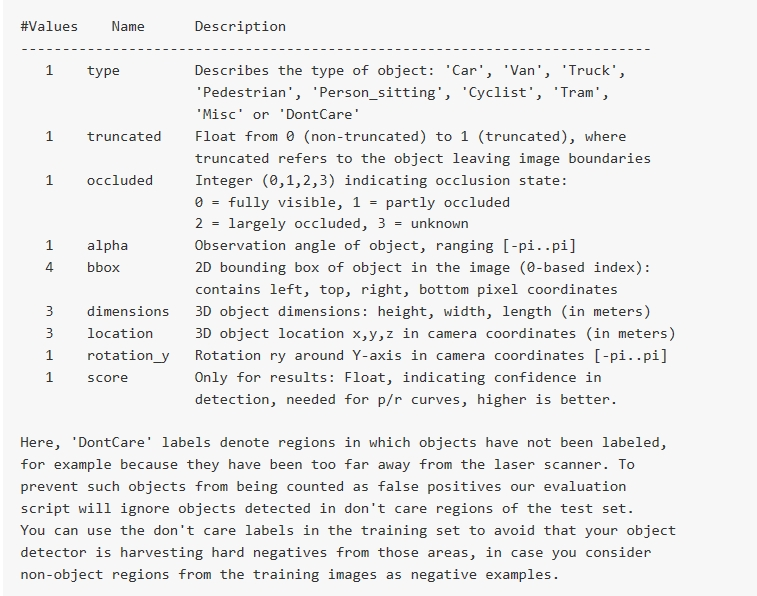
\includegraphics[width=5in]{images/KITTIForm.jpg}
	\caption{KITTI格式}
	\label{KITTIForm}
	\end{figure}
	KITTI数据集中共有7480张图片可以用来训练和测试。图\ref{KITTIForm}展示了KITTI数据集的典型样本,分为 ’Road’, ’City’, ’Residential’, ’Campus’ 和’Person’五类。原始数据采集于2011年的5天,共有180GB数据。

	\begin{figure}[htbp]
	\centering
	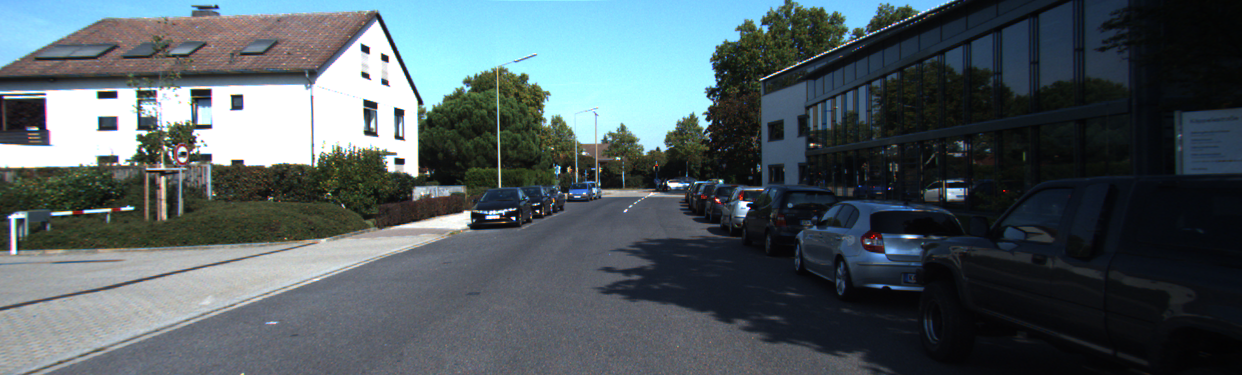
\includegraphics[width=5in]{images/007435.png}
	\caption{KITTI图像}
	\label{007435}
	\end{figure}
	数据图像如图\ref{007435},每张图片大小在1224*370左右。每张图片最多可显示15辆汽车和30名行人。

	\begin{figure}[htbp]
	\centering
	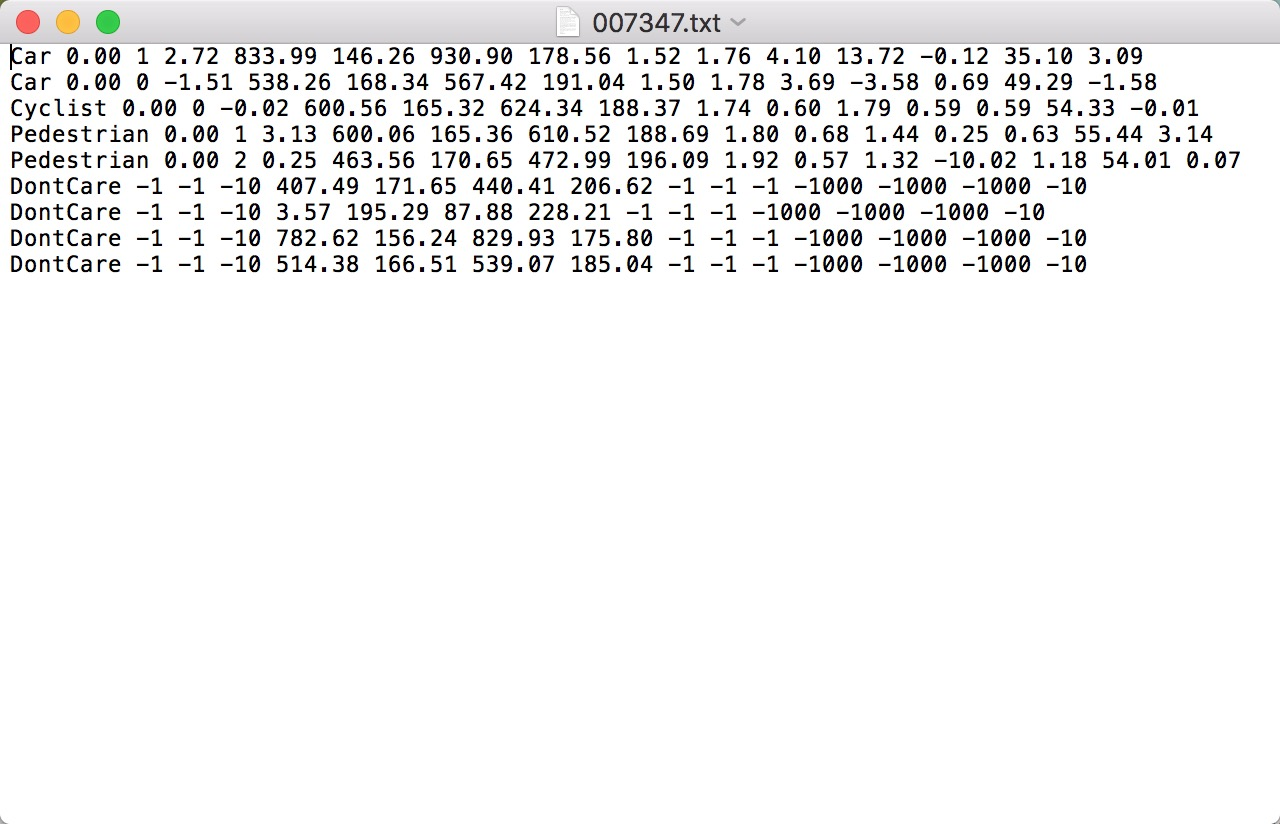
\includegraphics[width=5in]{images/KITTILable.png}
	\caption{KITTI标签}
	\label{KITTILable}
	\end{figure}
	数据标签如图\ref{KITTILable},每行是一个单独的物体。第一列是类名,而KITTI总共把所有的物体分了八个类(还有一个类名是DontCare,表示该区域没有被标注,防止假阳性);第二列代表物体超出边界多少;第三列表示物体被覆盖的情况;第四列是观察物体的角度;第五列到第八列是物体在图片中的位置(Xmin,Ymin,Xmax,Ymax);第九列到第十一列是三维物体的长宽高;第十二列到第十四列是三维物体在摄像机中的坐标(x,y,z),第十五列是物体在摄像机的坐标中离y轴的弧度。

	\subsection{数据转换和预处理}
	在实验过程中,我们将前7000张图片作为训练图片,后480张图片作为测试图片。

	\begin{figure}[htbp]
	\centering
	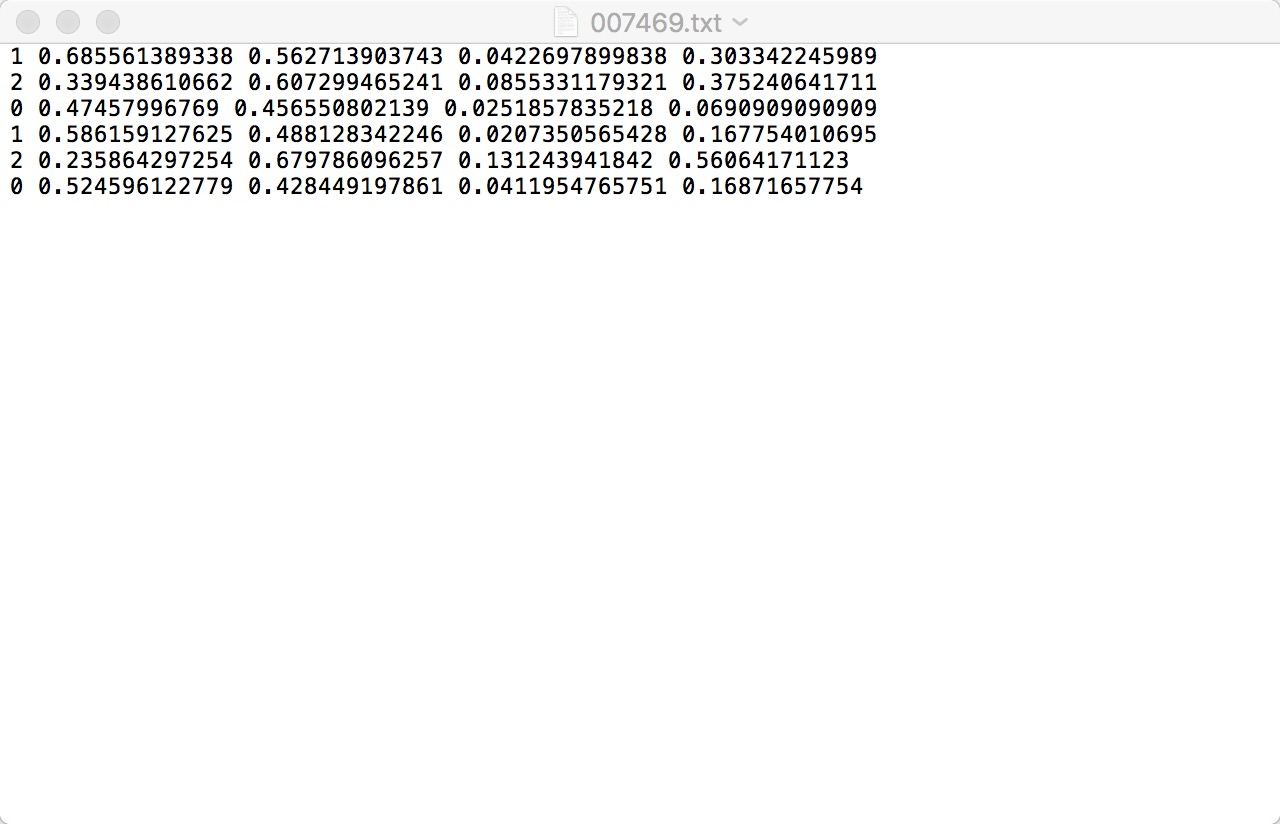
\includegraphics[width=5in]{images/darknetLabel.png}
	\caption{Darknet标签}
	\label{darknetLabel}
	\end{figure}
	首先,我们需要把数据集转换为Darknet所需要的形式,如图\ref{darknetLabel}。Darknet中:每行第一列是类的序号,第二列是框中心的x坐标,第三列是框中心的y坐标,第四列是框的宽度,第五列是框的高度。另外这四个数据都需要归一化到0-1之间。所以我们需要将KITTI标签中的(Xmin,Ymin,Xmax,Ymax)四个坐标进行下面的变换:

	$X = (X_{min} + X_{max}) / (2 * Weight)$

	$Y = (Y_{min} + Y_{max}) / (2 * Height)$

	$W = (X_{max} - X_{min}) / Weight$

	$H = (Y_{max} - Y_{min}) / Height$

	来变换到归一化后的(X,Y,W,H)。另外由于KITTI数据集中的类过多,我们适当调整为仅有三类:Car、Pedestrian、Cyclist,对应到0、1、2的标签。将原数据集中的Car、Van、Truck、Tram转换成Car;Pedestrian、Person\_sitting转换成Pedestrian;Cyclist转换成Cyclist;同时忽略掉Misc和DontCare的类。

	\begin{figure}[htbp]
	\centering
	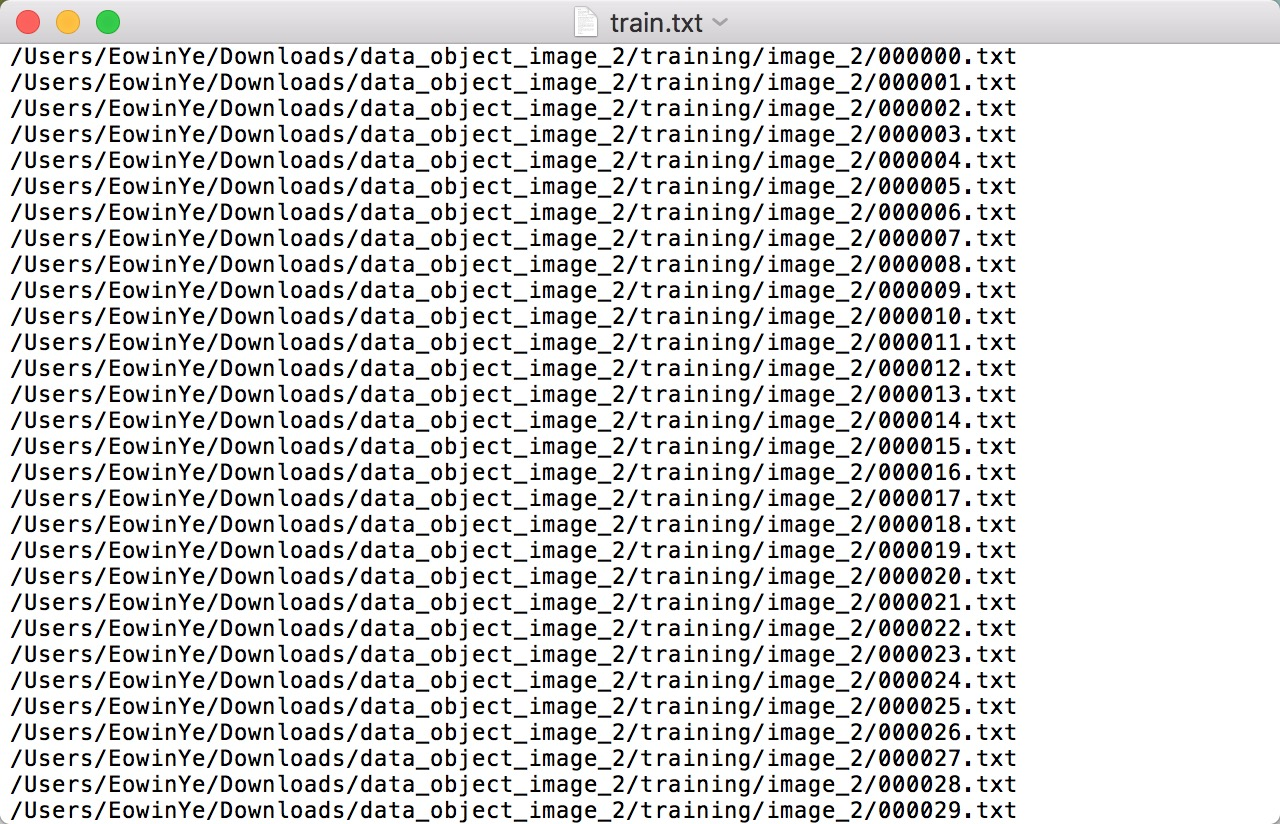
\includegraphics[width=5in]{images/trainList.png}
	\caption{Darknet标签}
	\label{trainList}
	\end{figure}
	然后,我们需要生存可以供Darknet读入的train\_list和test\_list,如图\ref{trainList}。这里直接将图片的前7000张作为训练图片,后480张作为测试图片然后生成对应的list文件即可。
}

\section{网络结构}{
网络结构参考YOLO的网络结构,在前面的章节我们已经讨论过YOLO的关键技术,这一节将主要讨论具体实现过程中的网络结构选择。

\subsection{损失函数}{
	损失函数是使用的平方误差。

	我们优化了模型输出中的平方误差。我们使用平方误差,因为它很容易优化,但是它不能完全符合我们的最大化平均精度的目标。我们增加了边界框坐标预测的损失,并减少了对不包含对象的框的置信预测的损失。我们使用两个参数,$\lambda_{coord}$和$\lambda_{noobj}$来完成这个。我们设置$\lambda_{coord}=5$和$\lambda_{noobj}=0.5$。平方误差也平等地对待大框和小框中的误差。 我们的误差度量应该反映出,大框中的小偏差比小框小。为了部分解决这个问题,我们直接预测边界框宽度和高度的平方根,而不是宽度和高度。

	在训练期间,我们优化以下多部分损失函数:
	\begin{eqnarray*}
	\lambda_{coord} \sum_{i=0}^{S^2} \sum_{j=0}^B 1_{ij}^{obj} (x_i - \hat{x_i})^2 + (y_i - \hat{y_i})^2 \\
	+ \lambda_{coord} \sum_{i=0}^{S^2} \sum_{j=0}^B 1_{ij}^{obj} (\sqrt{w_i} - \sqrt{\hat{w_i}})^2 + (\sqrt{h_i} - \sqrt{\hat{h_i}})^2 \\
	+ \sum_{i=0}^{S^2} \sum_{j=0}^B 1_{ij}^{obj} (C_i - \hat{C_i})^2 \\
	+ \lambda_{noobj} \sum_{i=0}^{S^2} \sum_{j=0}^B 1_{ij}^{noobj} (C_i - \hat{C_i})^2 \\
	+ \sum_{i=0}^{S^2} 1_{i}^{obj} \sum_{c \in classes} (p_i(c) - \hat{p_i}(c))^2
	\end{eqnarray*}

	其中$1_i^{obj}$表示如果对象出现在单元i中,并且$1_{ij}^{obj}$表示单元i中的第j个边界框预测器对于该预测是“负责的”。如果对象存在于该网格单元中,损失函数只会惩罚分类错误。 如果该预测因子对于真值框是“负责的”,则它也只对边界框坐标误差进行估计(即具有该网格单元中的任何预测变量的最高IOU)。
}

\subsection{完整网络结构YOLO}{
	\begin{figure}[htbp]
	\centering
	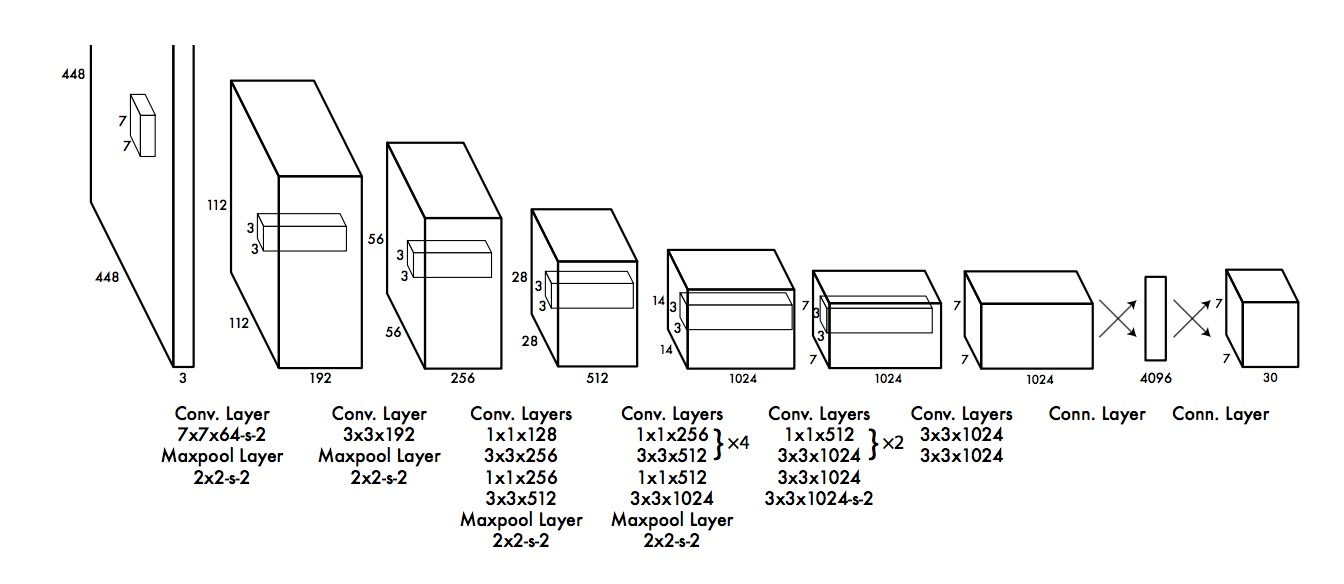
\includegraphics[width=5in]{images/net.png}
	\caption{完整网络结构YOLO}
	\label{net}
	\end{figure}
	如图\ref{net},参考YOLO和GoogLeNet模型\cite{googleNet},我们的网络有24个卷积层,其次是2个全连接层。部分卷积层后还连接了一些1*1的还原层。最后的卷积层使用了40个滤波器(num=5 * (class=3 + coords=4 + bias\_match=1))。除开最终层使用了线性激活函数,所有层使用以下leaky激活函数\ref{leaky}:
	\begin{figure}[htbp]
	\centering
	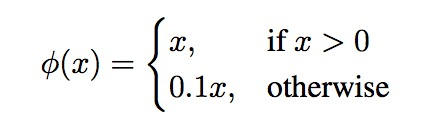
\includegraphics[width=5in]{images/leaky.png}
	\caption{leaky激活函数}
	\label{leaky}
	\end{figure}

	该网络比较大,实际训练过程中所需显存较多,训练出来的模型参数更多,理论上效果也会更好,不过速度会偏慢。
}

\subsection{缩小网络结构tiny-YOLO}{
	针对速度的要求,我们又采用了一种tiny-YOLO的网络来进行试验。

	tiny-YOLO仅有9个卷积层,并且每个卷积层使用了更少的滤波器(输出的特征),其它网络结构和之前的网络结构一样。理论上来说,tiny-YOLO将实现非常快速度的检测,同时模型大小也将降低不少,不过将造成部分精度的损失。
}
}

\section{验证方法}{
	本项目将采用计算各个类别的AP(Average Precision)的方法实现对检测结果的评估\cite{VOC}。

	\begin{figure}[htbp]
	\centering
	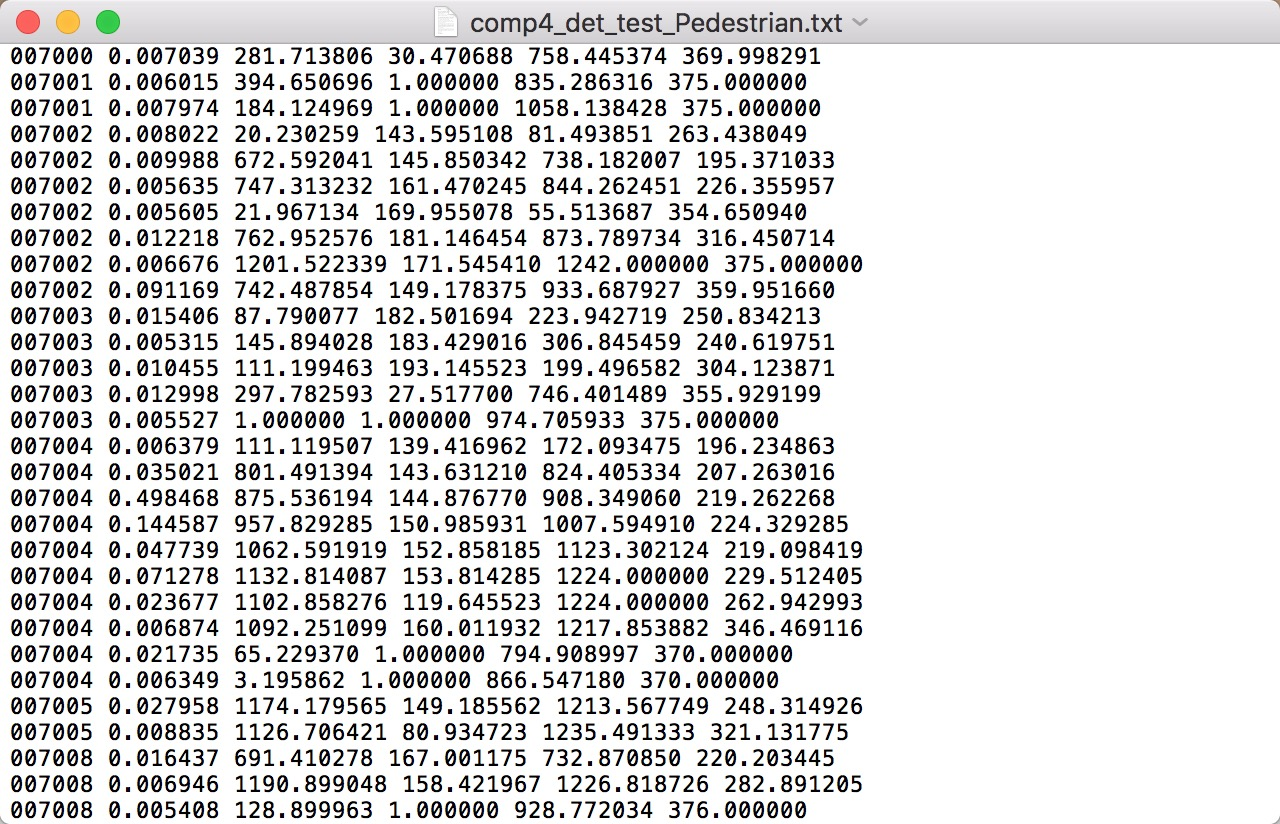
\includegraphics[width=5in]{images/results.png}
	\caption{行人验证结果}
	\label{results}
	\end{figure}
	训练好的模型对于每张图片会返回各个框的检测结果(x,y,w,h,class,precision)。而在实际验证中,每个类别会返回所有大于阈值的检测结果,如图\ref{results}。每种类都有单独的文件存放检测结果,文件形式为(img\_id, Xmin, Ymin, Xmax, Ymax, score)。我们就需要用这个检测结果和原标签对比,得到最终的实验结果。

	对于每个类,AP的具体算法如下:

	1.按照预测结果的score将预测结果按降序排序。

	2.对于每个预测结果$(\hat{X}_{min},\hat{Y}_{min},\hat{X}_{max},\hat{Y}_{max})$,找到所对应的文件中该类的各个真值$({X}_{imin},{Y}_{imin},{X}_{imax},{Y}_{imax})$,计算覆盖量IOU

	$$intersection = (max(\hat{X}_{min},{X}_{imin}) - min(\hat{X}_{max},{X}_{imax})) * (max(\hat{Y}_{min},{Y}_{imin}) - min(\hat{Y}_{max},{Y}_{imax}))$$

	$$union = (\hat{X}_{max} - \hat{X}_{min}) * (\hat{Y}_{max} - \hat{Y}_{min}) + ({X}_{imax} - {X}_{imin}) * ({Y}_{imax} - {Y}_{imin}) - intersection$$

	$$IOU = union / intersection$$

	3.更新TP(true positive),FP(false positive):选取匹配的真值中IOU最高的IOU。如果IOU大于阈值(0.5)并且该真值没有被检测到过TP就加一,否则FP加一。

	4.计算AP值:做出PR曲线,找到score降序的数组中,所有TP加一的位置,然后将这些位置i乘以前i个预测的准确率,再求和
	$$AP = \sum_{IOU>thresh}1*pre(i) / N$$其中N是真值的数量。
}

\section{本章小结}{
	本章主要讲述了本项目的整体研究流程。首先从数据集的处理上分析了KITTI数据集的特征,以及转换成YOLO所需的格式的数据预处理等;接着,我们讨论了该项目网络的损失函数,分析了所使用的各种网络结构;最后,我们讨论了测试结构的格式以及相对应的验证方法AP。
}


  \chapter{实验结果与分析}
本章将对实验进行检验并对比分析:将统计各个类的AP值并做出PR曲线;预测效果展示,并展现其中效果不佳的结果;探究实验泛化性能力。
\section{实验平台}{
	基本环境:
	\begin{enumerate}
		\item 操作系统: CentOS Linux release 7.1
		\item 显卡: GTX1080
		\item CUDA版本: 8.0
		\item 实验框架: Darknet
		\item 数据集: KITTI
	\end{enumerate}

	YOLO训练参数:
	\begin{enumerate}
		\item batch size: 64
		\item width: 416
		\item height: 416
		\item channels: 3
		\item momentum: 0.9
		\item decay: 0.0005
		\item learing rate: 0.001
		\item max batches: 50000
	\end{enumerate}

	tiny-YOLO训练参数:
	\begin{enumerate}
		\item batch size: 64
		\item width: 416
		\item height: 416
		\item channels: 3
		\item momentum: 0.9
		\item decay: 0.0005
		\item learing rate: 0.001
		\item max batches: 50000
	\end{enumerate}

	如图\ref{trainYOLO}、\ref{trainTiny-YOLO},展现了两个模型的训练过程。

	\begin{figure}[htbp]
	\centering
	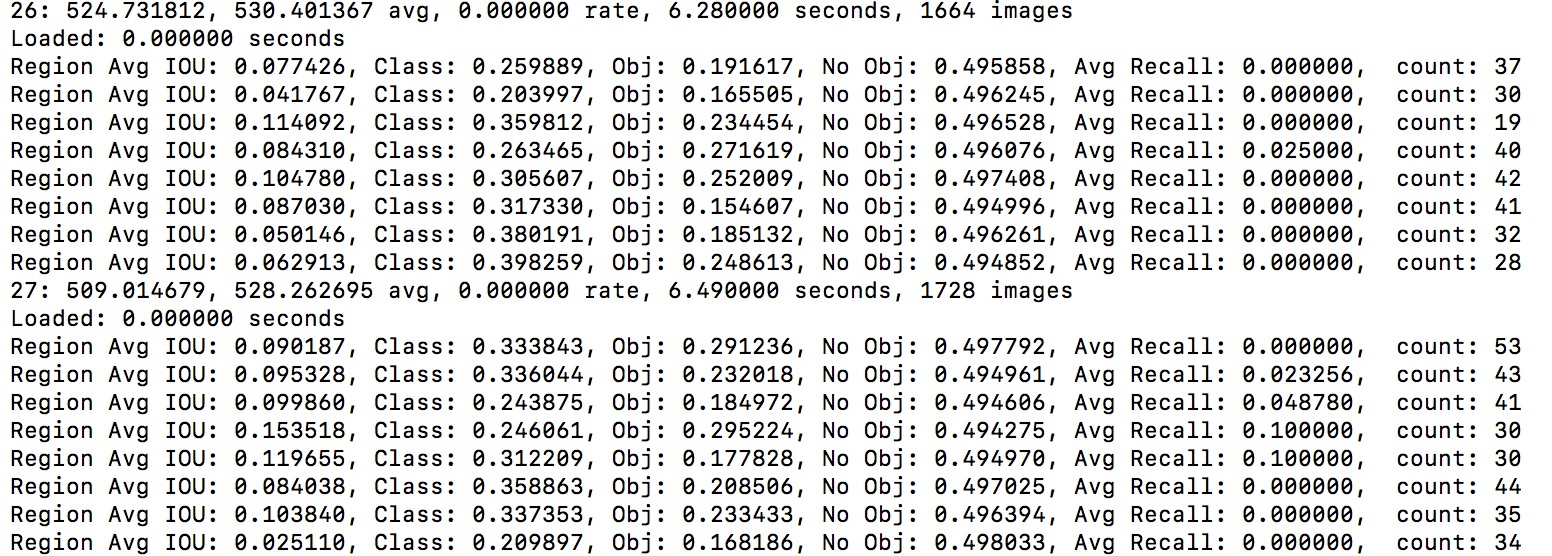
\includegraphics[width=5in]{images/trainYOLO.png}
	\caption{YOLO训练过程}
	\label{trainYOLO}
	\end{figure}
	\begin{figure}[htbp]
	\centering
	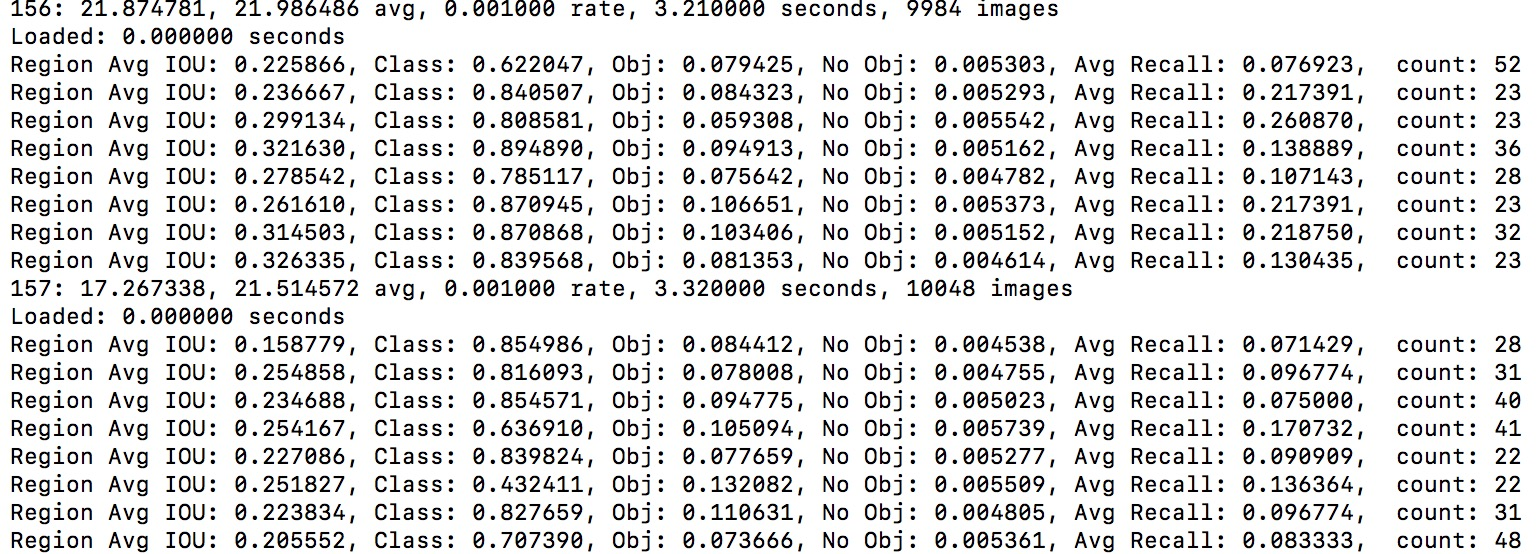
\includegraphics[width=5in]{images/trainTiny-YOLO.png}
	\caption{tiny-YOLO训练过程}
	\label{trainTiny-YOLO}
	\end{figure}
}

\section{结果对比}{
	\subsection{AP比较}
	\begin{table}  
	\caption{各模型各类AP和FPS结果对比}  
	\begin{tabular}{l|p{2cm}p{2cm}p{2cm}p{2cm}}  
	\hline  
	             & Pedestrian & Car      & Cyclist  & FPS \\  
	\hline  
	Faster R-CNN & 65.91 \%   & 79.11 \% & 62.81 \% & 5   \\  
	YOLO         & 51.44 \%   & 68.05 \% & 50.97 \% & 45  \\
	tiny-YOLO    & 26.67 \%   & 50.75 \% & 25.04 \% & 120 \\
	\hline
	\end{tabular}
	\label{AP}
	\end{table} 
	我们首先对比本项目各个模型对于各个类的AP值以及FPS比较,如表\ref{AP}。其中Faster R-CNN的数据参考自\cite{KITTI}。

	通过图表,我们可以发现虽然tiny-YOLO有120fps,而yolo只有45fps,比YOLO的速度快上2-3倍,但是性能远不如YOLO。从速度上来看,YOLO能达到每秒45帧的速度,已经基本可以满足实时行人检测的需求,tiny-YOLO甚至然能够达到每秒120帧的速度,两个模型均能满足实时行人检测的要求。从性能上来看,不管是哪个类的AP值,YOLO都全面领先于tiny-YOLO,尤其是在行人和自行车的检测上,而YOLO不仅在行人和自行车上能分别达51.44AP和50.97AP,在车辆检测上更是能达到68.05AP,效果较好。而反观tiny-YOLO,它在车辆检测上只有50.75AP,而在行人检测和自行车检测上更是仅有26.67AP和25.04AP

	从整体上看,模型对车辆的检测明显高于对行人和自行车的检测,这是由于KITTI数据集中车辆数据较多造成的。而模型的整体表现也部分受限于训练数据过少。

	对比Faster R-CNN,Faster R-CNN仅有5fps,无法满足实时行人检测的要求,不管是YOLO还是tiny-YOLO,在速度上都明显比Faster R-CNN要快上很多。并且Faster R-CNN在行人、车辆、自行车上的检测分别有65.91AP、79.11AP、62.81AP,YOLO在这三项上的损失并没有想象上的那么大。可见YOLO仅牺牲了部分的精度确在检测速度上提高了很多。

	总的来说,YOLO在AP上的表现达到预期效果,而tiny-YOLO虽然速度很快,但是效率上损失过多。

	\subsection{PR曲线比较}
	\begin{figure}[htbp]
	\centering
	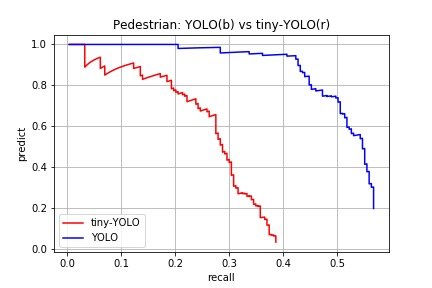
\includegraphics[width=5in]{images/pedestrianPR.png}
	\caption{行人检测比较}
	\label{pedestrianPR}
	\end{figure}
	\begin{figure}[htbp]
	\centering
	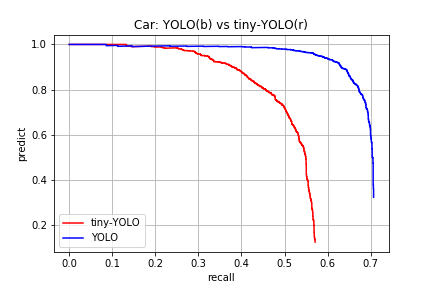
\includegraphics[width=5in]{images/carPR.png}
	\caption{车辆检测比较}
	\label{carPR}
	\end{figure}
	\begin{figure}[htbp]
	\centering
	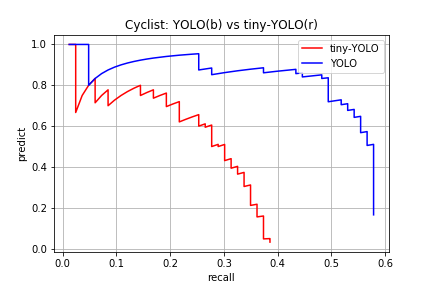
\includegraphics[width=5in]{images/cyclistPR.png}
	\caption{自行车检测比较}
	\label{cyclistPR}
	\end{figure}
	我们分别对各个模型各个类做出PR曲线并进行比较,结果如图\ref{pedestrianPR}、\ref{carPR}、\ref{cyclistPR}。

	从图\ref{pedestrianPR}中可以看出,对于行人的检测上,YOLO模型明显好于tiny-YOLO的模型,在召回率0.4的时候,tiny-YOLO的准确率已经接近0,而YOLO的准确率还是接近1。

	从图\ref{carPR}中可以看出,对于车辆的检测,两个模型都有很好的表现,PR曲线都很飘。tiny-YOLO大概在召回率大于0.45后准确率开始快速下降,而YOLO则在召回率大于0.6后准确率快速下降。

	从图\ref{cyclistPR}中可以看出,对于自行车的检测,YOLO模型也明显好于tiny-YOLO模型。tiny-YOLO下降速度比较稳定,而YOLO在召回率大于0.5后准确率开始快速下降。
}

\section{预测效果}{
	\subsection{效果展示}
	\begin{figure}[htbp]
	\centering
	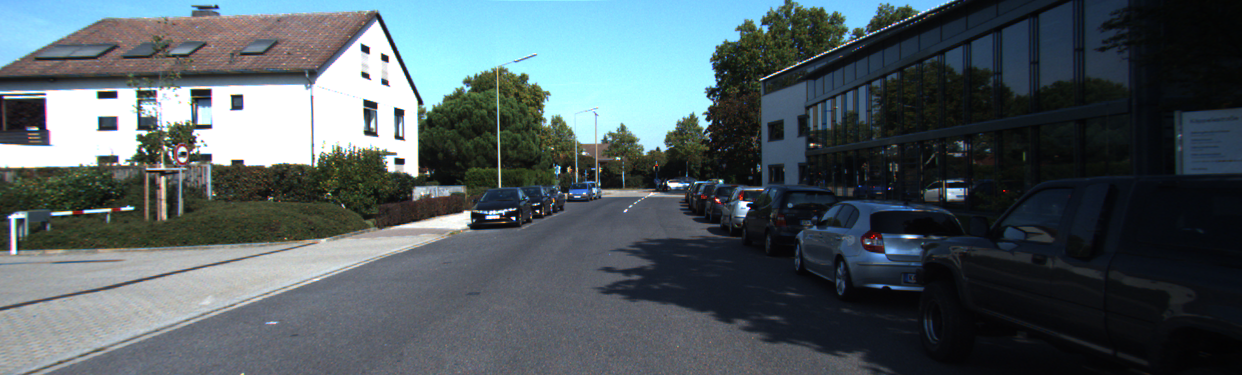
\includegraphics[width=5in]{images/007435.png}
	\caption{输入图像}
	\label{007435}
	\end{figure}
	我们选择了一张情形较为复杂的图作为输入,如图\ref{007435}。

	\begin{figure}[htbp]
	\centering
	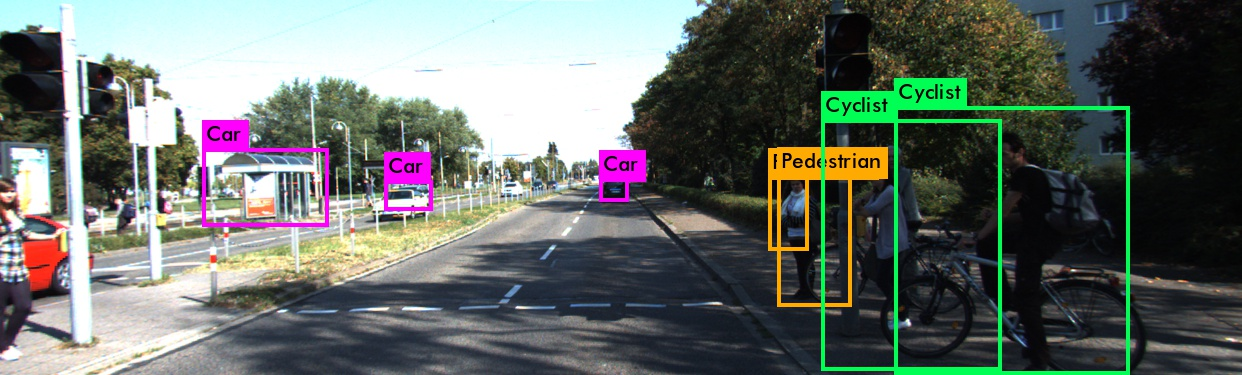
\includegraphics[width=5in]{images/predictYOLO.jpg}
	\caption{YOLO预测结果}
	\label{predictYOLO}
	\end{figure}
	\begin{figure}[htbp]
	\centering
	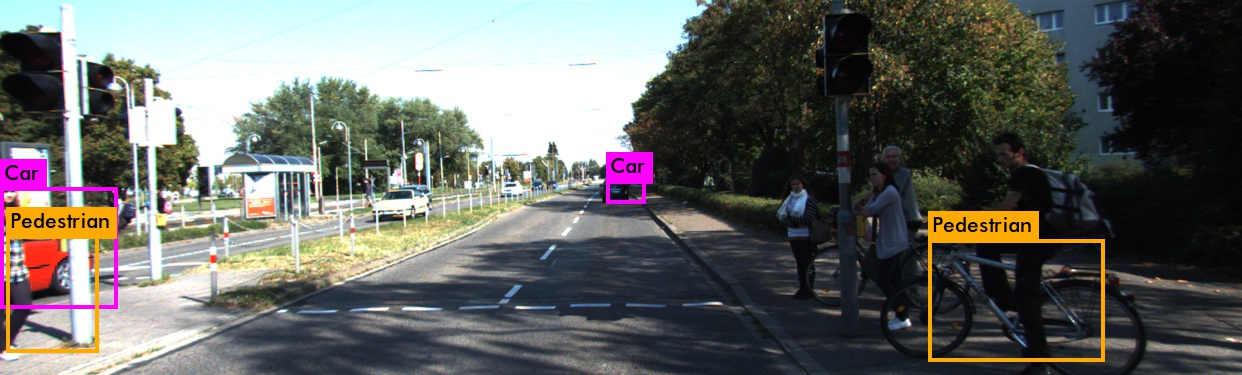
\includegraphics[width=5in]{images/predictTiny-YOLO.jpg}
	\caption{tiny-YOLO预测结果}
	\label{predictTiny-YOLO}
	\end{figure}

	测试结果如图\ref{predictYOLO}、\ref{predictTiny-YOLO}所示。YOLO的测试结果中,预测出来的结果基本正确,而且预测框很好的覆盖了物体,不过其中出现了两个错误,一个是重复预测了一个行人,一个是将公交车站预测成为了车辆;另外一些不完整的车辆和行人没有预测出来。而tiny-YOLO的情况就较为差了,很大一部分容易预测出来的物体并没有成功检测到,将自行车预测成行人,预测框与物体的真值框差别较大。

	从上述分析中我们可以看出YOLO基本能满足行人检测的要求,而tiny-YOLO的检测性能过低就不太适合了。另外使用YOLO网络对不完整的物体检测性能不佳,有重复检测情况,对过于细小的物体检测不佳(大部分模型对过于细粒度物体的检测都不太支持)。

	\subsection{错误结果分析}
	我们分别检测了YOLO模型在细小物体靠的近时候的表现以及不完整物体的表现。

	\begin{figure}[htbp]
	\centering
	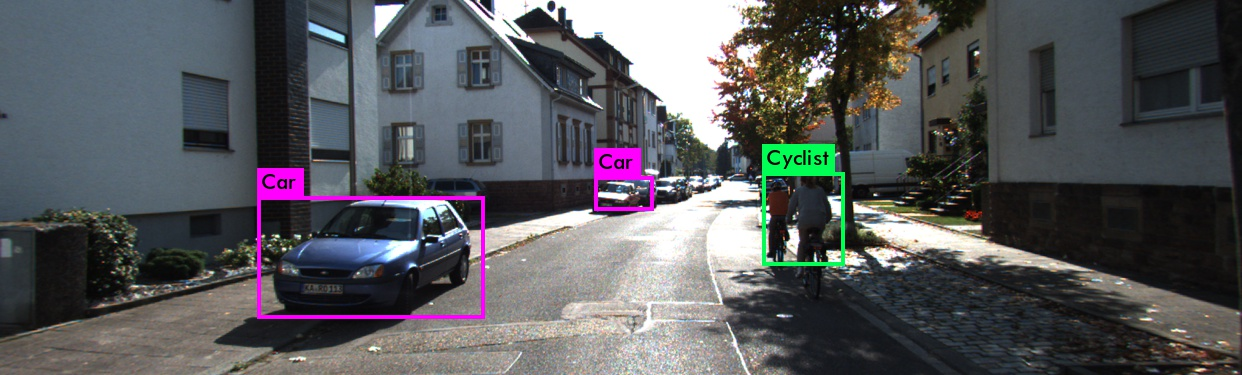
\includegraphics[width=5in]{images/error1.jpg}
	\caption{细小集群的测试}
	\label{error1}
	\end{figure}
	如图\ref{error1},YOLO队友两个靠的很近骑自行车的人检测成了一个骑自行车的人,这主要是由于YOLO将物体检测分为了S*S的方格,而多个细粒度的物体如果在一个方格内的话,YOLO会很容易将多个物体检测成一个物体。所以YOLO对细粒度的集群检测性能不佳。

	\begin{figure}[htbp]
	\centering
	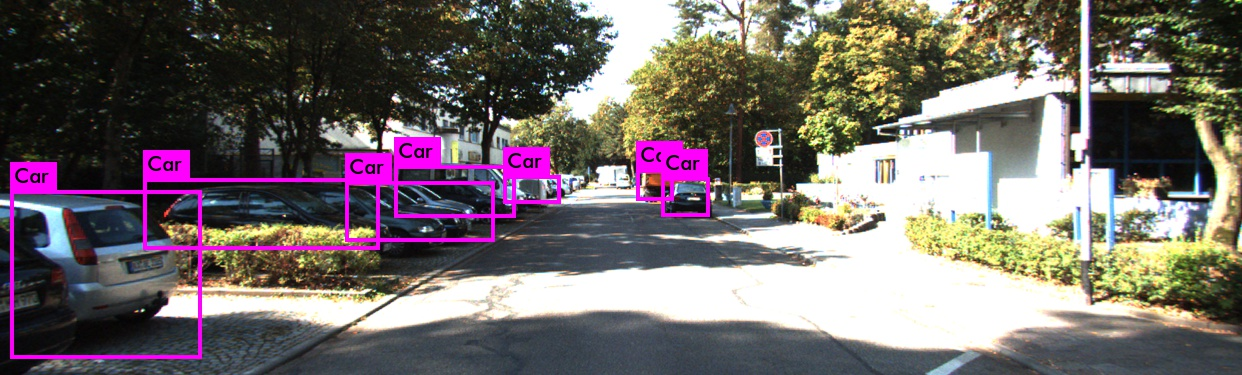
\includegraphics[width=5in]{images/error2.jpg}
	\caption{不完整物体的测试}
	\label{error2}
	\end{figure}
	如图\ref{error2},YOLO对不完整物体的检测没有想象中的糟糕,对于大部分不完整的物体还是能够准确检测出来的,除开该物体残缺部分过多。另外由于YOLO对细小集群表现不佳,物体间的覆盖也会导致检测的性能损失。

	\begin{figure}[htbp]
	\centering
	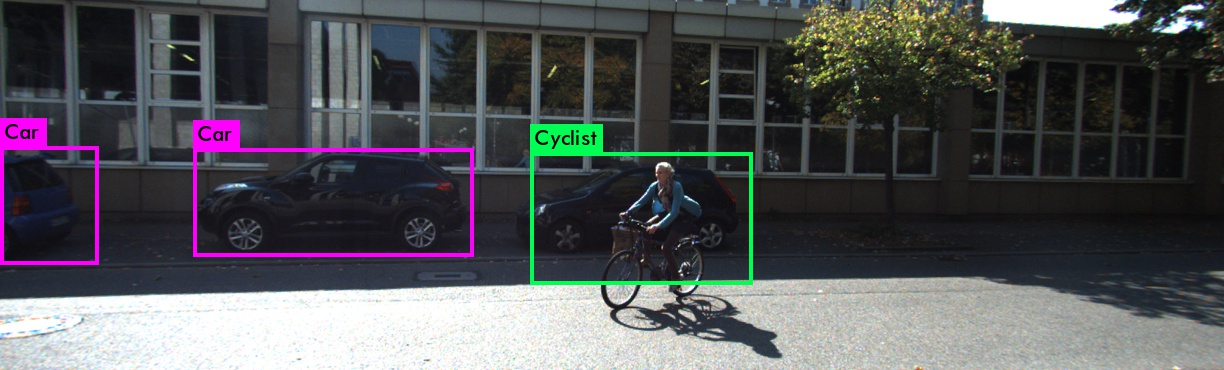
\includegraphics[width=5in]{images/error3.jpg}
	\caption{不同物体覆盖的测试}
	\label{error3}
	\end{figure}
	如图\ref{error3},YOLO对不同物体的覆盖检测性能不佳。该问题与YOLO对细小集群检测不佳的问题类似,这是由于YOLO把检测问题分为S*S的方格,而每个方格只预测其中一个具体的类,如果不同物体产生覆盖现象,往往不能同时预测成功出这些不同的物体来。
}

\section{泛化性}{
	本项目讨论实时行人检测的可行性,针对日常生活驾驶、极端天气、夜晚等各种情形进行实验。

	\begin{figure}[htbp]
	\centering
	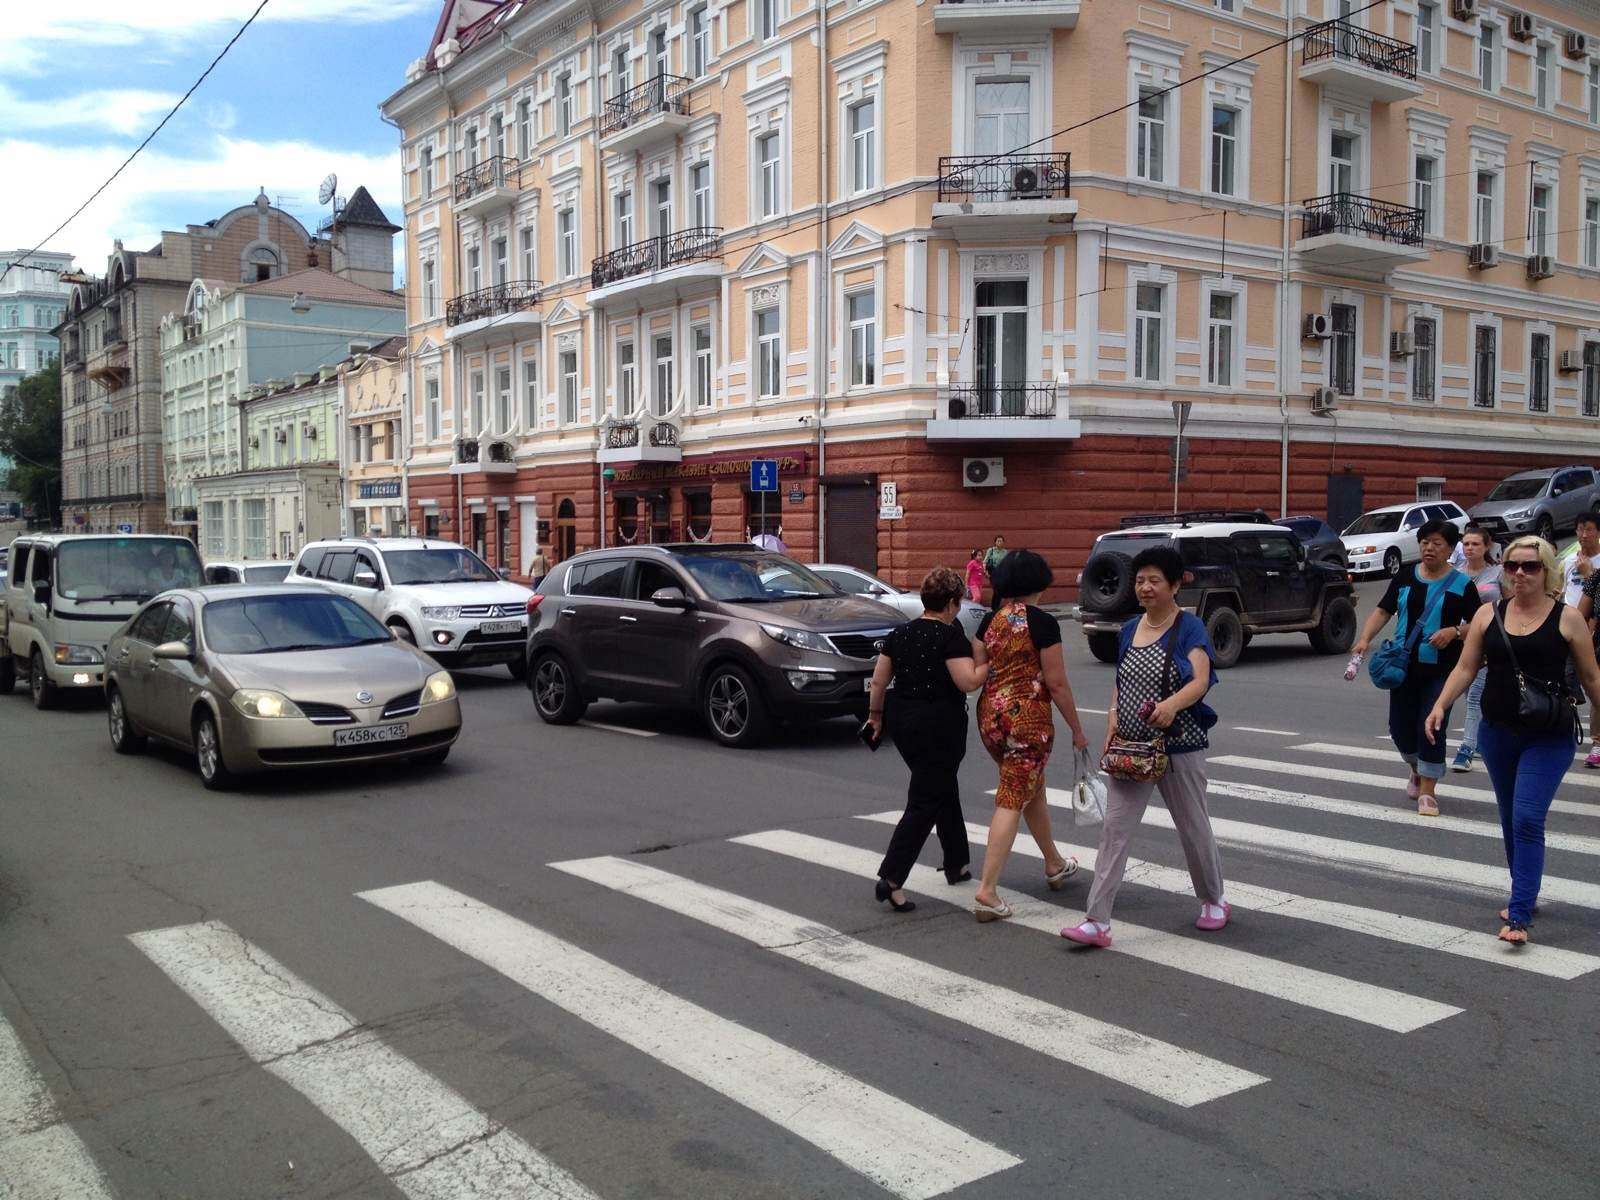
\includegraphics[width=5in]{images/daily.jpg}
	\caption{日常生活驾驶}
	\label{daily}
	\end{figure}
	\begin{figure}[htbp]
	\centering
	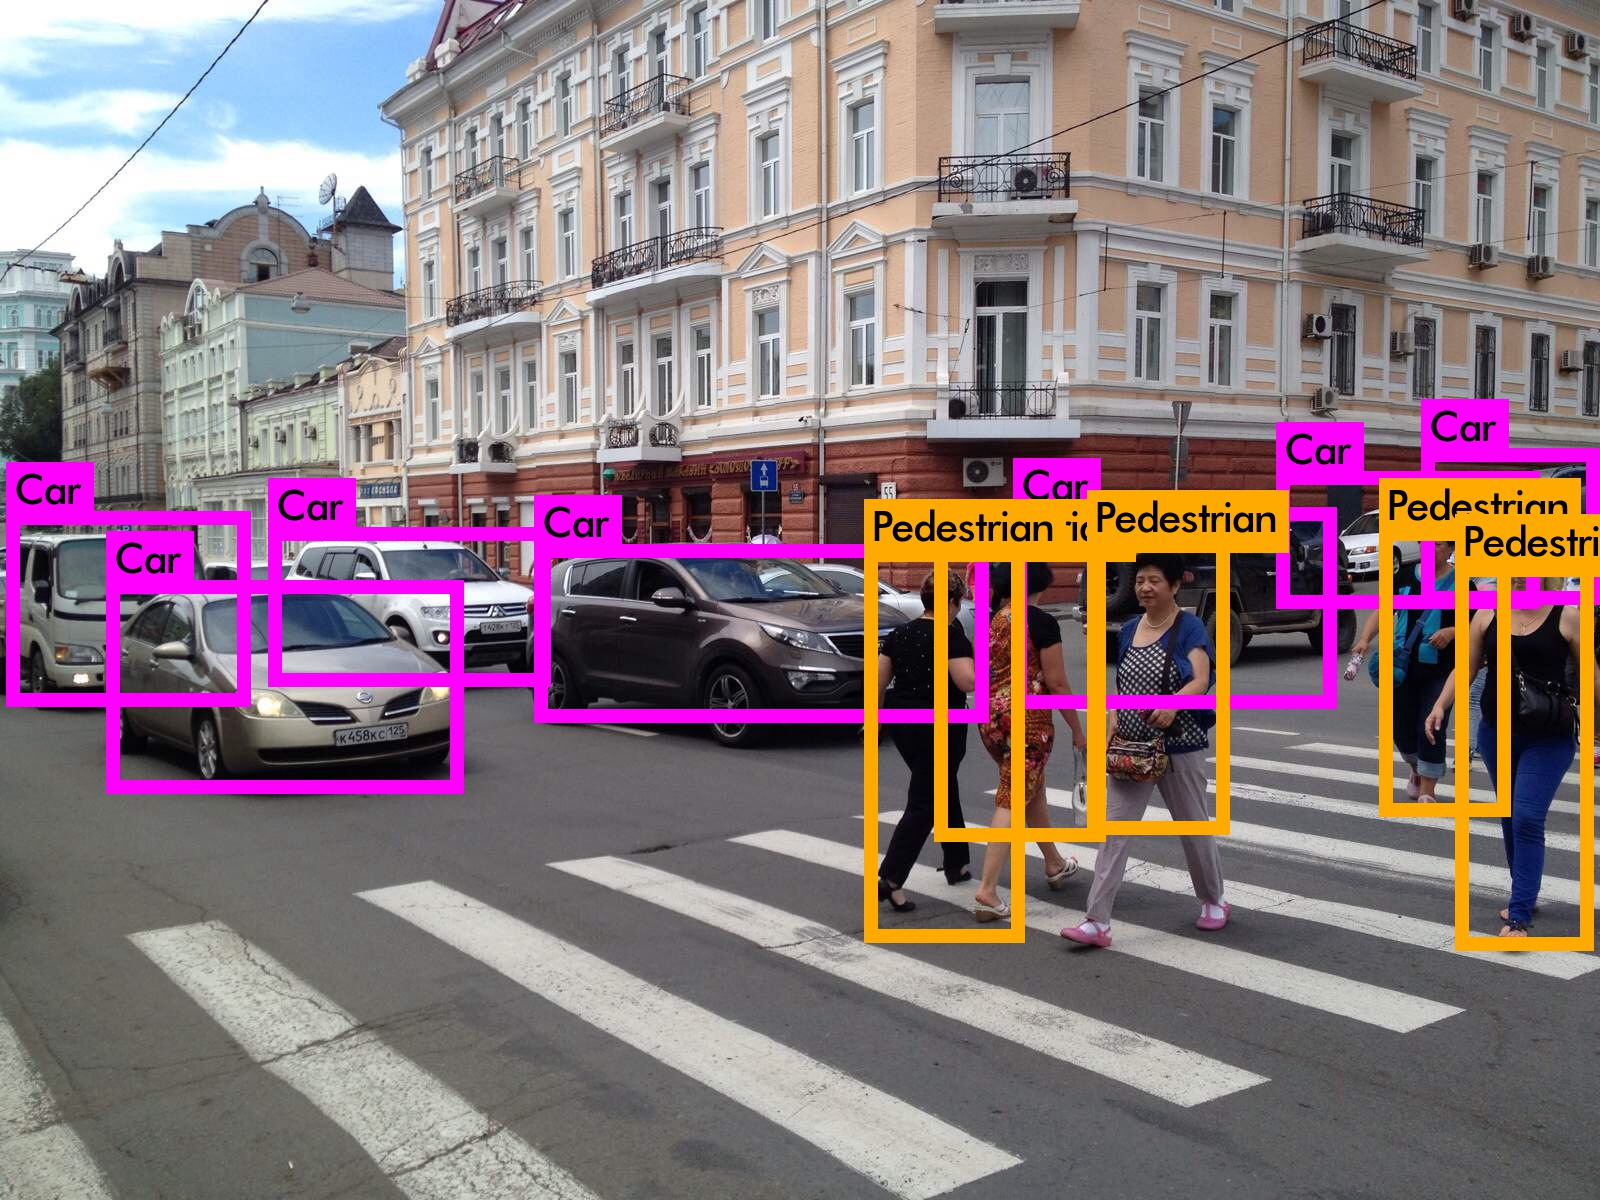
\includegraphics[width=5in]{images/predictDaily.jpg}
	\caption{日常生活驾驶预测结果}
	\label{predictDaily}
	\end{figure}
	我们针对日常生活驾驶过程中的情况做了测试,测试输入如图\ref{daily},预测结果如图\ref{predictDaily}。模型对正常驾驶情况下的预测性能很好,基本能够满足实时行人检测的要求。

	\begin{figure}[htbp]
	\centering
	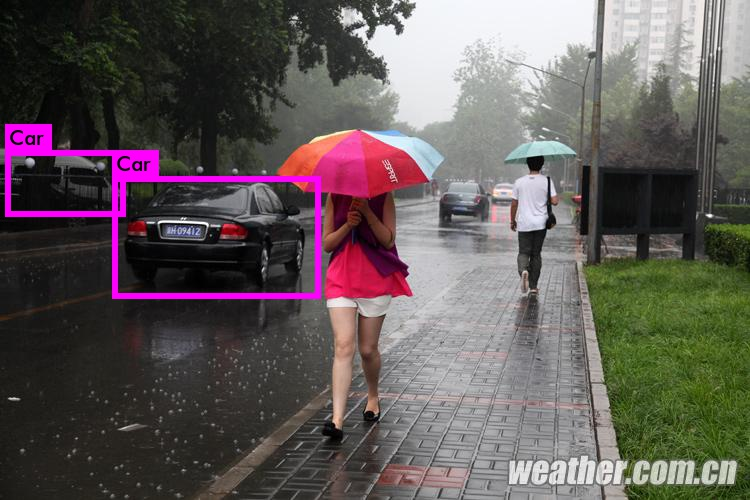
\includegraphics[width=5in]{images/rain.jpg}
	\caption{雨中行人检测}
	\label{rain}
	\end{figure}
	\begin{figure}[htbp]
	\centering
	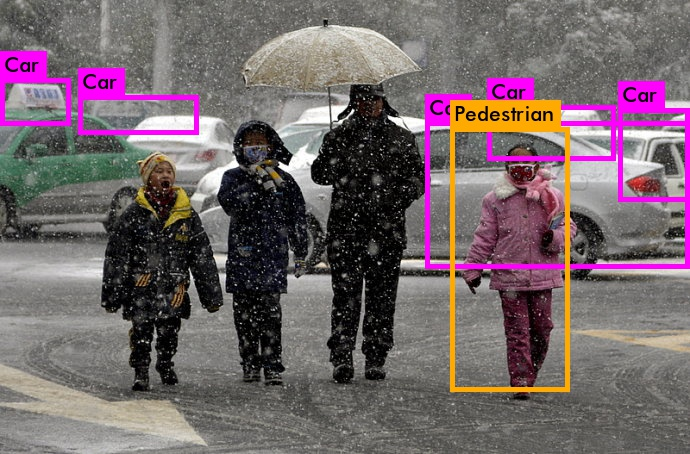
\includegraphics[width=5in]{images/snow.jpg}
	\caption{雪中行人检测}
	\label{snow}
	\end{figure}
	我们针对极端天气情况进行了泛化性测试,结果如图\ref{rain}、\ref{snow}。从图中可以看出,模型对极端天气情况下表现较差,对于雪中的预测,可能是主要受到噪声(雪)的干扰,所以行人和车辆预测效果都不佳;对于雨中的预测,则可能是受到行人拿伞的影响,所以对行人检测性能不佳但是对车辆检测性能还行。

	\begin{figure}[htbp]
	\centering
	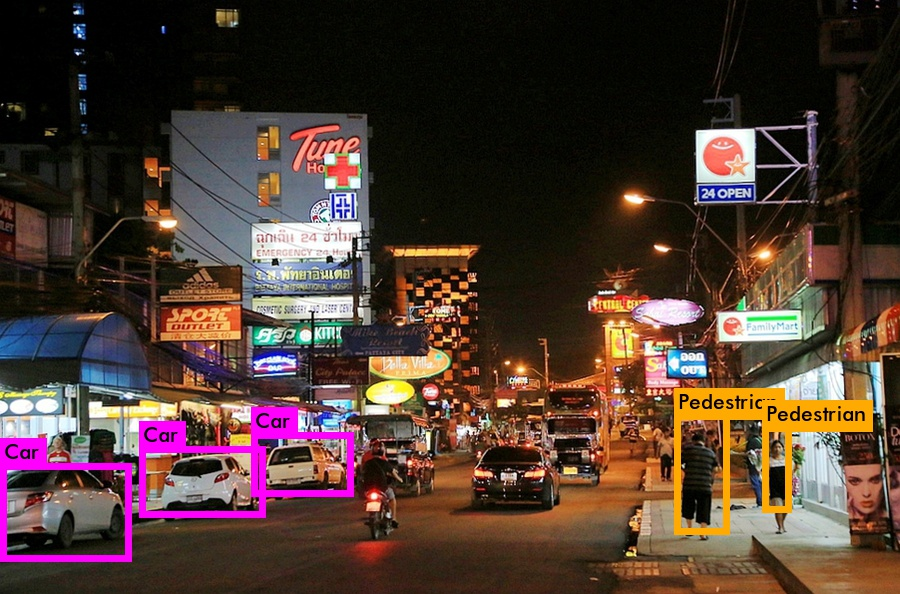
\includegraphics[width=5in]{images/night.jpg}
	\caption{夜晚行人检测}
	\label{night}
	\end{figure}
	我们针对夜晚的情况进行了泛化性测试,结果如图\ref{night}。从图中可以看出,模型对夜晚情况下行人和车辆的检查性能还行,虽然还是远不如正常情况下的行人检测,但是已经能够说明模型能在夜晚或光照不好的情况下进行行人检测。
}

\section{本章小结}{
	本章对本项目做了详细的实验和分析。我们首先介绍了我们的实验环境和训练参数等。接着,我们研究了各个模型的AP、FPS值和PR曲线,对比分析得到YOLO网络基本满足实时行人检测的要求。之后我们具体分析了预测的效果以及错误结果的分析,分析出了YOLO进行行人检测的一些弊端。最后我们对模型进行了泛化性的检验,检验结果表明虽然对于极端天气情况下模型表现不佳,但是总体而言模型的泛化性程度较高。通过实验,我们探究了模型的实时行人检测的能力和不足。
}



  \chapter{分析与讨论}

\section{第一节}

\section{本章小结}



  \chapter{本文总结}

\section{工作成果总结}{
	整个项目完成了面向实时行人检测的卷积神经网络的研究,并分析对比了各个模型的实验结果。描述了使用YOLO网络作为实时行人检测的研究方案,分析了YOLO最后的表现与性能。

	搭建了Darknet的深度学习框架,学习了Darknet的使用方法,参考了Darknet的源码来满足实验的需求。

	使用了KITTI数据集作为本项目的训练和测试数据集,介绍了KITTI数据集的形式,通过预处理数据将KITTI数据集转换为YOLO所需的形式,并划分为训练、测试数据,供之后YOLO网络训练和测试使用。

	调整了网络结构,分别参考了YOLO和tiny-YOLO的网络结构来进行实验。基于Darknet框架完成了整个模型的训练和测试过程。

	验证了实验结果,通过AP、PR曲线等方法对比分析了各模型实验结果,最后的实验结果也基本符合预期效果,而YOLO的网络结构更是不仅在速度上达到了令人满意的程度,模型性能也相对较好。

	综上所述,本项目基本完成了预期的研究成果,同时也对未来的研究有所启迪。
}

\section{未来工作}{
	当前研究的不足之处在于:

	1.受限于算法问题,模型对于细小集群的检测性能不佳。

	2.受限于算法问题,模型对于不同小物体覆盖时检测性能不佳。

	3.受限于训练数据等影响,模型对于极端天气条件和夜晚泛化性不佳。

	对于面向实时行人检测的卷积神经网络的研究,还可以继续完善的工作如下:

	1.改进模型。测试深度学习模型,如SSD、Faster R-CNN在行人检测上的性能和速度。

	2.尝试其他数据集。针对其他不同的行人数据集分别进行训练和测试,研究不同数据集下各个模型的表现。

	3.增强模型的泛化性。尝试提取图像特征,或优化采样策略针对特殊场景进行训练以提高模型对不同场景、天气、夜晚的泛华性。

	4.采用二值化网络来进行网络的训练和测试\cite{RAR}。近来深度学习网络二值化是一个火热的话题,使用二值化网络理论上可以大大减少网络的大小,大大加快网络的传递速度,未来可以尝试从这个方向研究实时行人检测。
}


%==============================================================
%这也是个不需要自己修改的部分。

  \backmatter %结束章节自动编号

  %参考文献
  \addcontentsline{toc}{chapter}{参考文献} % 解决目录中没有相应的参考文献的条目问题
  \chaptermark{参考文献}

%==============================================================

  \bibliography{data/zjubib}

  %致谢
  %致谢
\chapter*{\centerline{致\quad 谢}}
\chaptermark{致谢}
\addcontentsline{toc}{chapter}{致谢}

\vspace{2em}


  %附录
  \chapter*{附\quad 录}
\chaptermark{附录}
\addcontentsline{toc}{chapter}{附录} 


  %任务书
  %任务书
\chapter*{\centerline{\stxingkai\erhao 本科生毕业论文(设计)任务书}}
\thispagestyle{empty}

\vspace{2em}

{\stfangsong\xiaosi\bf
一、\;题目:\; \uline{面向实时行人检测的快速卷积神经网络\hfill\hspace{4mm}}

二、\;指导教师对毕业论文(设计)的进度安排及任务要求:

进度安排:三月底前提交开题报告(含文献翻译,文献综述);四月到五月完成实验研究,撰写论文;五月底前提交完整的论文和报告;六月六日前毕业论文定稿并完成答辩准备工作

任务要求:毕业论文要求本科生在充分理解并掌握某专业理论和技术的基础上,完成某一科研(子)课题的研究和实现,并对个人工作进行总结,按照科学论文的规范撰写成文。


\begin{flushright}
起讫日期 2017 \quad 年 3 \quad 月 1 \quad 日 至 2017 \quad 年 5 \quad 月 \quad 30 日\\
指导教师(签名)\;\underline{\hspace{4em}} \quad 职称\;\underline{\hspace{4em}}
\end{flushright}

三、\;系或研究所审核意见:
\vspace{2cm}
\begin{flushright}
负责人(签名)\underline{\hspace{4em}}\\
\quad 年 \quad 月 \quad 日
\end{flushright}
}

  %考核
  %考核
\chapter*{\centerline{\stfangsong\xiaoer 毕~业~论~文~(设计)~考~核}}
\thispagestyle{empty}

\vspace{2em}

{\stfangsong\sihao\bf
一、\;指导教师对毕业论文(设计)的评语:
\vspace{4cm}

\begin{flushright}
    指导教师(签名)\;\underline{\hspace{4em}}\\
    年\quad 月\quad 日
\end{flushright}

二、\;答辩小组对毕业论文(设计)的答辩评语及总评成绩:
\vspace{4cm}

{\songti\xiaosi
\begin{tabular}{|c|c|c|c|c|c|}
    \hline
    成绩比例 & \parbox[t]{4em}{文献综述\\[-3.5em]占(10\%)} & 
               \parbox[t]{4em}{开题报告\\[-3.5em]占(20\%)} & 
               \parbox[t]{4em}{外文翻译\\[-3.5em]占(10\%)} &
               \parbox[t]{7em}{毕业论文(设计)\\[-3.5em]质量及答辩\\[-3.5em]占(60\%)} & 
               总评成绩 \\
    \hline
    分值 & & & & & \\
    \hline
\end{tabular}
}

\begin{flushright}
    答辩小组负责人(签名)\;\underline{\hspace{4em}}\\
    年 \quad 月 \quad 日
\end{flushright}
}


%==============================================================
%==============================================================
\end{document}
